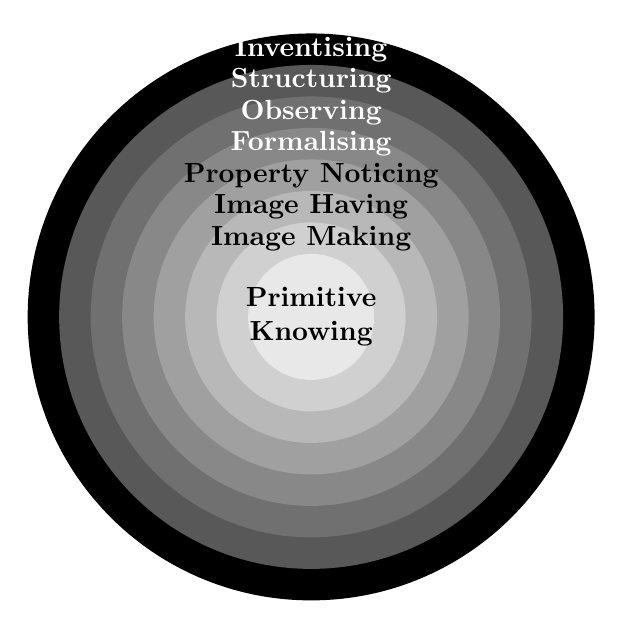
\begin{tikzpicture}
  % Define colors for each layer (grayscale from light to dark)
  \definecolor{layer1}{RGB}{232,232,232}
  \definecolor{layer2}{RGB}{208,208,208}
  \definecolor{layer3}{RGB}{184,184,184}
  \definecolor{layer4}{RGB}{160,160,160}
  \definecolor{layer5}{RGB}{136,136,136}
  \definecolor{layer6}{RGB}{112,112,112}
  \definecolor{layer7}{RGB}{88,88,88}
  \definecolor{layer8}{RGB}{0,0,0}
  
  % Draw concentric circles from outermost to innermost
  \fill[layer8] (0,0) circle (3.6cm);
  \fill[layer7] (0,0) circle (3.2cm);
  \fill[layer6] (0,0) circle (2.8cm);
  \fill[layer5] (0,0) circle (2.4cm);
  \fill[layer4] (0,0) circle (2.0cm);
  \fill[layer3] (0,0) circle (1.6cm);
  \fill[layer2] (0,0) circle (1.2cm);
  \fill[layer1] (0,0) circle (0.8cm);
  
  % Add labels
  \node[font=\bfseries] at (0,0) {\begin{tabular}{c}Primitive\\Knowing\end{tabular}};
  \node[font=\bfseries] at (0,1.0) {Image Making};
  \node[font=\bfseries] at (0,1.4) {Image Having};
  \node[font=\bfseries] at (0,1.8) {Property Noticing};
  \node[font=\bfseries,white] at (0,2.2) {Formalising};
  \node[font=\bfseries,white] at (0,2.6) {Observing};
  \node[font=\bfseries,white] at (0,3.0) {Structuring};
  \node[font=\bfseries,white] at (0,3.4) {Inventising};
\end{tikzpicture}
